\documentclass[a4paper,12pt]{article}
\setcounter{tocdepth}{4}

% \usepackage[latin1]{inputenc}
\usepackage[utf8]{inputenc} 
\usepackage[italian]{babel}
\usepackage{indentfirst}
\usepackage[margin=2.2cm]{geometry}
\usepackage[most]{tcolorbox}
\usepackage{graphicx}
\usepackage{subcaption}
\usepackage{hyperref}
\usepackage[italian]{varioref}
\usepackage{listings}
\usepackage{xcolor}
\usepackage[numbered,framed]{matlab-prettifier}
\usepackage[font={small}]{caption}
\usepackage{xcolor}

\usepackage{tikz}
\usetikzlibrary{arrows.meta}
\usetikzlibrary{shapes}
\usetikzlibrary{positioning}
\tikzset{%
  every neuron/.style={
    circle,
    draw,
    minimum size=1cm
  },
  neuron missing/.style={
    draw=none, 
    scale=4,
    text height=0.333cm,
    execute at begin node=\color{black}$\vdots$
  },
}

\captionsetup[figure]{labelfont={bf},name={Figura},labelsep=period}

\renewcommand*{\fullref}[1]{\hyperref[{#1}]{\vref*{#1}, \emph{\nameref*{#1}}}}
\newcommand*{\coderef}[1]{\hyperref[{#1}]{\nameref*{#1} a pagina \pageref*{#1}}}

\renewcommand{\textfraction}{0}
\renewcommand{\topfraction}{1}
\renewcommand{\bottomfraction}{1}
\renewcommand{\floatpagefraction}{1}

\graphicspath{{figures/}}


\title{\textbf{Fashion MNIST -- Rete Naurale per il Riconoscimento di Immagini di Capi di Abbigliamento}}
\author{Lara Vignotto}
\date{\today}  


\begin{document}

\maketitle

\vfill
\tableofcontents


%%%%%%%%%%%%%%%%%%%%%%%%%%%%%%
\newpage
\section{Presentazione e scopi del progetto}
Lo scopo di questo progetto è la realizzazione, l'analisi e la documentazione di una rete neurale per la classificazione di immagini di capi di abbigliamento provenienti dall'archivio Fashion MNIST. Ogni immagine ha dimensione $28\times28$ pixel ed è rappresentata in scala di grigi. Il lavoro è diviso nelle seguenti sezioni:
\begin{itemize}
    \item Nel \textbf{secondo capitolo} presenteremo le specifiche del modello di rete neurale adottato e l'architettura che ne deriva;
    \item Nel \textbf{terzo capitolo} daremo una panoramica sulla struttura del software, espondendo i moduli che compongono il pacchetto;
    \item Nel \textbf{quarto capitolo} verrà descritta brevemente la procedura dedicata alla preparazione dei dati;
    \item Il \textbf{quinto capitolo} sarà dedicato alla procedura relativa alla fase di apprendimento;
    \item Nel \textbf{sesto capitolo} riporteremo il codice;
    \item Nel \textbf{settimo capitolo} presenteremo i risultati;
    \item Nell'\textbf{ottavo capitolo} discuteremo i risultati mostrati al capitolo precedente.
\end{itemize}




\newpage
%%%%%%%%%%%%%%%%%%%%%%%%%%%%%%
\section{Modello e architettura della rete} % cap2

La rete neurale è composta da tre strati (Figura~\vref{fig:modello}):
\begin{itemize}
    \item Un \emph{input layer} di 784 nodi, che corrispondono ai $28\times28$ pixel di ciascuna immagine;
    \item Un \emph{hidden layer} di 100 nodi con funzione di attivazione ReLU;
    \item Un \emph{output layer} di 10 nodi con funzione di attivazione softmax, uno per ogni categoria, ovvero le dieci classi di capi di abbigliamento.
\end{itemize}

\begin{figure}[htb]
    \centering
    \tcbox[boxrule=.3mm,colback=white]{
% tikz picture from
% https://tex.stackexchange.com/a/153974
\begin{tikzpicture}[x=2cm, y=1.5cm, >=stealth]

    \foreach \m/\l [count=\y] in {1,2,3,missing,4}
    \node [every neuron/.try, neuron \m/.try] (input-\m) at (0,2.5-\y) {};

    \foreach \m [count=\y] in {1,missing,2}
    \node [every neuron/.try, neuron \m/.try ] (hidden-\m) at (2,2-\y*1.25) {};

    \foreach \m [count=\y] in {1,missing,2}
    \node [every neuron/.try, neuron \m/.try ] (output-\m) at (4,1.5-\y) {};

    \foreach \l [count=\i] in {1,2,3,784}
    \draw [<-] (input-\i) -- ++(-1,0)
        node [above, midway] {$I_{\l}$};

    \foreach \l [count=\i] in {1,100}
    \node [] at (hidden-\i) {$H_{\l}$};

    \foreach \l [count=\i] in {1,10}
    \draw [->] (output-\i) -- ++(1,0)
        node [above, midway] {$O_{\l}$};

    \foreach \i in {1,...,4}
    \foreach \j in {1,...,2}
        \draw [->] (input-\i) -- (hidden-\j);

    \foreach \i in {1,...,2}
    \foreach \j in {1,...,2}
        \draw [->] (hidden-\i) -- (output-\j);

    \foreach \l [count=\x from 0] in {Input, Hidden, Ouput}
    \node [align=center, above] at (\x*2,2) {\l \\ layer};

\end{tikzpicture}
    }
    \caption{Schema della rete neurale.}\label{fig:modello}
\end{figure}





\newpage
%%%%%%%%%%%%%%%%%%%%%%%%%%%%%%
\section{Struttura del software} % cap3

Il pacchetto per questa rete neurale è composto da otto moduli, ovvero 1 script e 7 funzioni:
\begin{itemize}
    \item La funzione \texttt{FashionMNIST\_DataPrep} per la preparazione dei dati;
    \item La funzione \texttt{processImagesFashionMNIST}, procedura di lettura e decodifica delle immagini;
    \item La funzione \texttt{processLabelsFashionMNIST}, procedura di decodifica delle etichette (categorie);
    \item Lo script \texttt{FashionMNIST\_Training} per la definizione dell'architettura di rete, l'impostazione dell'apprendimento e la valutazione di prestazioni;
    \item La funzione \texttt{FashionMNIST\_DeltaRule} che applica la regola di apprendimento;
    \item La funzione \texttt{label2matrix} per convertire un insieme di etichette in forma matriciale;
    \item La funzione di attivazione \texttt{Softmax};
    \item La funzione di attivazione \texttt{ReLU}.
\end{itemize}


\begin{figure}[htb]
    \centering
    \tcbox[boxrule=.3mm,colback=white]{
\begin{tikzpicture}
    \node (a) [draw,rectangle,rounded corners] 
    {\texttt{processImagesFashionMNIST}};
    \node (b) [xshift=6cm,draw,rectangle,rounded corners] 
    {\texttt{processLabelsFashionMNIST}};
    \node (c) [xshift=6.5cm,yshift=-1cm,draw,draw,rectangle,rounded corners] 
    {\texttt{Softmax}};
    \node (d) [xshift=10cm,yshift=-1cm,draw,draw,rectangle,rounded corners] 
    {\texttt{ReLU}};
    \node (e) [xshift=1.5cm,yshift=-3cm,draw,rectangle,rounded corners] 
    {\texttt{FashionMNIST\_DataPrep}};
    \node (f) [xshift=8cm,yshift=-3cm,draw,rectangle,rounded corners] 
    {\texttt{FashionMNIST\_DeltaRule}};
    \node (g) [xshift=4.5cm,yshift=-5cm,draw,rectangle,rounded corners] 
    {\texttt{FashionMNIST\_Training}};
    \node (h) [xshift=-2cm,yshift=-1cm,draw,rectangle,rounded corners] 
    {\texttt{label2matrix}};

    \draw   [-{Latex[length=3mm]}] (a)--(e);        
    \draw   [-{Latex[length=3mm]}] (b)--(e);
    \draw   [-{Latex[length=3mm]}] (c)--(f);        
    \draw   [-{Latex[length=3mm]}] (d)--(f);
    \draw   [-{Latex[length=3mm]}] (e)--(g);       
    \draw   [-{Latex[length=3mm]}] (f)--(g);
    \draw   [-{Latex[length=3mm]}] (h)--(e);
\end{tikzpicture}
    }
    \caption{Schema dei moduli software e legami tra loro.}
    \label{fig:schema-software}
\end{figure}



\newpage
%%%%%%%%%%%%%%%%%%%%%%%%%%%%%%
\section{Preparazione dei dati} % cap4
\label{sec:preparazione}

Descriviamo qui in breve le singole parti in cui è strutturata la procedura \texttt{fashionMNIST\-\_\-Da\-ta\-Prep} (pagina~\pageref{lst:dataprep}).

\paragraph{(a) L'archivio dei dati.}
Fashion-MNIST è un dataset di immagini degli articoli di abbigliamento della società di vendita di vestiti online Zalando. È costituito da un \emph{training set} di 60 000 immagini e un \emph{test set} di 10 000 immagini. Ogni \emph{sample} è un'immagine in scala di grigi di dimensione $28\times28$ pixel, associata a un'etichetta $0-9$ corrispondente ad una delle 10 classi (dalle t-shirt agli stivali). 

È simile al dataset MNIST in quanto condivide le stesse dimensioni delle immagini e la stessa struttura della divisione tra insieme di addestramento e di test.


\paragraph{(b) Lettura e decodifica dei dati.}
La funzione \texttt{fashionMNIST\-\_\-Da\-ta\-Prep} richiama le funzioni di processamento \texttt{processImagesFashionMNIST} e \texttt{processLabelsFashionMNIST} (pagine~\pageref{lst:processimages} e~\pageref{lst:processlabels}) per caricare i dati di immagini ed etichette per costruire \emph{training set} e \emph{validation set}. 

Queste funzioni estraggono i dati dai file IDX scaricati e inseriscono le immagini in \texttt{dlarray} a quattro dimensioni (altezza immagine, larghezza immagine, livelli di grigio, numero di immagine), e le etichette in array contenente i valori $0-9$ delle categorie assegnati ad ogni immagine. Maggiori informazioni sono riportate nel capitolo \fullref{sec:codice}.

\paragraph{(c) Esplorazione dei dati.}
Successivamente la funzione permette di visualizzare un insieme casuale di 20 immagini del \emph{training set} in un'unica figura. L'immagine è stata riportata nel capitolo \fullref{sec:risultati}.


\paragraph{(d) Splitting dei dati.}
Infine, viene fatto manualmente lo splitting dei dati. Abbiamo raggruppato tutte e 70 000 le immagini (sia di \emph{training} che di \emph{validation}) in un'unica variabile, e lo stesso è stato fatto per le etichette. In quest'ultimo caso è stata richiamata la funzione \texttt{labels2matrix} (pagina~\pageref{lst:label2matrix}) per convertire la variabile delle etichette in forma matriciale, ovvero in una matrice le cui righe sono vettori di dieci elementi: nove 0, e un 1 in posizione della classe corretta.

Successivamente abbiamo specificato la percentuale di splitting per poi effettuarlo con la funzione \texttt{randperm()}. La funzione \texttt{fashionMNIST\-\_\-Da\-ta\-Prep} restituisce gli insiemi di immagini ed etichette per il \emph{training} e gli insiemi di immagini ed etichette per la \emph{validation}.





\newpage
%%%%%%%%%%%%%%%%%%%%%%%%%%%%%%
\section{Procedura di apprendimento} % cap5
\label{sec:apprendimento}

Descriviamo qui in breve le singole parti in cui è strutturata la procedura \texttt{fashionMNIST\-\_\-Trai\-ning} (pagina~\pageref{lst:training}).

\paragraph{(a) Settaggio dei parametri e inizializzazione dei pesi.}
Lo script inizializza il \emph{learning rate}, gli insiemi di \emph{training} e \emph{test}, e successivamente i pesi degli archi tra strato di \emph{input} e strato nascosto, e tra strato nascosto e strato di \emph{output}.


\paragraph{(b) Applicazione della delta rule.}
Lo script richiama la funzione \texttt{fashionMNIST\-\_\-Del\-ta\-Rule} (pagina~\pageref{lst:deltarule}). La \emph{delta rule} viene applicata ad ogni epoca, e consiste in una fase di \emph{feedforward} e una di \emph{backpropagation} per l'aggiornamento dei pesi. La funzione restituisce le matrici dei pesi aggiornati e una matrice di \emph{output} relativa all'addestramento della rete.


\paragraph{(c) Stima dell’errore MSE e visualizzazione delle curve.}
Durante l'apprendimento calcoliamo l'errore MSE ad ogni epoca. Le curve \emph{loss} risultanti al variare del \emph{learning rate} e del numero di epoche sono riportati al calpitolo \fullref{sec:risultati}.




\newpage
%%%%%%%%%%%%%%%%%%%%%%%%%%%%%%
\section{Codice} % cap6
\label{sec:codice}

\begin{lstlisting}[style=Matlab-editor,title=\texttt{FashionMNIST\_DataPrep.m},label=lst:dataprep]
function [TrainImgs, TrainLabels, TestImgs, TestLabels] = FashionMNIST_DataPrep()
%   Caricamento delle immagini da Fashion MNIST
    filenameImagesTrain = 'fashion/train-images-idx3-ubyte';
    filenameLabelsTrain = 'fashion/train-labels-idx1-ubyte';
    filenameImagesTest = 'fashion/t10k-images-idx3-ubyte';
    filenameLabelsTest = 'fashion/t10k-labels-idx1-ubyte';

    XTrain = processImagesFashionMNIST(filenameImagesTrain);
    YTrain = processLabelsFashionMNIST(filenameLabelsTrain);
    XTest = processImagesFashionMNIST(filenameImagesTest);
    YTest = processLabelsFashionMNIST(filenameLabelsTest);
%
%   Visualizzazione di un insieme casuale delle immagini
    figure
    perm = randperm(60000,20);
%
    for i = 1:20
        subplot(4, 5, i);
        images = extractdata(XTrain(:,:,1,:));
        imshow(images(:,:,1,perm(i)));
    end
%
%%%%%%%%%%%%%%%%%%% Raggruppamento
%   Numero totale delle immagini contenute negli archivi
    numtotImages = 70000;
%  
%   Inizializzazione degli array
    images = zeros(28,28,numtotImages);
    labels = zeros(numtotImages, 1);
%
%   Raggruppamento delle immagini delle etichette
    images(:,:,1:60000) = extractdata(XTrain);
    images(:,:,60001:numtotImages) = extractdata(XTest);
    labels(1:60000,:) = YTrain;
    labels(60001:numtotImages,:) = YTest;
%
%   La variabile labels e' convertita in forma matriciale
%   tramite la funzione label2matrix.   
    labels = label2matrix(labels);
%   
%%%%%%%%%%%%%%%%%%% Splitting
%   Percentuale di splitting
    training_perc = 0.8; 
%   Randomizzazione degli indici delle immagini
    split_perm = randperm(numtotImages);
%   Cardinalita' dell'insieme di apprendimento (training)
    training_cardin = floor(numtotImages * training_perc);

%   Cardinalita' dell'insieme di collaudo (validation)
    validation_cardin = numtotImages - training_cardin;   

%   Definizione degli insiemi di apprendimento 
%   e delle relative etichette, tutti randomizzati
    TrainImgs=images(:,:,split_perm(1:training_cardin));
    TrainLabels=labels(split_perm(1:training_cardin),:);
%   Definizione degli insiemi di collaudo 
%   e delle relative etichette, tutti randomizzati
    ValidationImgs = ...
        images(:,:,split_perm(training_cardin+1:end));
    ValidationLabels = ... 
        labels(split_perm(training_cardin+1:end),:);
%
end
\end{lstlisting}



\newpage
\begin{lstlisting}[style=Matlab-editor,title=\texttt{processImagesFashionMNIST.m},label=lst:processimages]
function X = processImagesFashionMNIST(filename)
%   Apre in lettura il file IDX di immagini 
    [fileID,errmsg] = fopen(filename,'r','b');
%   Controlla se il file puo' essere aperto correttamente
    if fileID < 0   % fopen non e' riuscito a aprire il file
        error(errmsg);
    end

%   Legge i dati da file binario e ottiene il magic number 
%   leggendo i primi 4 bytes. 
    magicNum = fread(fileID,1,'int32',0,'b');
    if magicNum == 2051 % Magic number per le immagini
        fprintf('\nRead fashion MNIST image data...\n')
    end

%   Legge i successivi 3 set di 4 bytes, che ritornano 
%   il numero di immagini, righe e colonne
    numImages = fread(fileID,1,'int32',0,'b'); % Num di imgs
    fprintf('Number of images in the dataset: %6d ...\n', ... 
        numImages);
    numRows = fread(fileID,1,'int32',0,'b'); % Num di righe
    numCols = fread(fileID,1,'int32',0,'b'); % Num di colonne

%   Legge i dati di immagine
    X = fread(fileID,inf,'unsigned char');

%   Fa il reshape dell'array e scambia le prime due dimensioni
%   perche' i dati sono stati letti per colonna
    X = reshape(X,numCols,numRows,numImages);
    X = permute(X,[2 1 3]);
%   Divide i valori dei pixel per 255 per normalizzare nel range [0,1] 
    X = X./255;
    X = reshape(X, [28,28,1,size(X,3)]); % Forma di matrice
    X = dlarray(X, 'SSCB'); % Converte l'array 3-D in un dlarray 4-D

    fclose(fileID); % Chiude il file
end
\end{lstlisting}


\newpage
\begin{lstlisting}[style=Matlab-editor,title=\texttt{processLabelsFashionMNIST.m},label=lst:processlabels]
function Y = processLabelsFashionMNIST(filename)
%   Apre in lettura il file IDX di etichette
    [fileID,errmsg] = fopen(filename,'r','b');
%   Controlla se il file puo' essere aperto correttamente
    if fileID < 0   % fopen non e' riuscito a aprire il file
        error(errmsg);
    end

%   Legge i dati da file binario e ottiene il magic number 
%   leggendo i primi 4 bytes.
    magicNum = fread(fileID,1,'int32',0,'b');
    if magicNum == 2049 % Magic number per le etichette
        fprintf('\nRead fashion MNIST label data...\n')
    end

    numItems = fread(fileID,1,'int32',0,'b'); % Num di labels
    fprintf('Number of labels in the dataset: %6d ...\n', ... 
        numItems);

%   Array contenente i valori 0-9 delle etichette
    Y = fread(fileID,inf,'unsigned char');

    fclose(fileID); % Chiude il file
end
\end{lstlisting}



\vfill
\begin{lstlisting}[style=Matlab-editor,title=\texttt{label2matrix.m},label=lst:label2matrix]
function matrix = label2matrix(label)
%
%   Conversione di formato di un'etichetta per avere         
%   categorie numerate da 1 a 10 e non da 0 a 9
    label(label == 0) = 10;
%   Inizializzazione delle matrici
    matrix = zeros(length(label),10);
%
    for i = 1:length(label)
        matrix(i, label(i)) = 1;
    end
%
    end  %  fine della function
\end{lstlisting}




\newpage
\begin{lstlisting}[style=Matlab-editor,title=\texttt{FashionMNIST\_Training.m},label=lst:training]
clear
alpha = 0.01;
[TrainImgs, TrainLabels, ValidationImgs, ValidationLabels] = ... 
    FashionMNIST_DataPrep();
%
% Inizializzazione casuale dei pesi
w1 = 2 * rand(100, 784) - 1; % input > hidden
w2 = 2 * rand(10, 100) - 1;  % hidden > output
%
%   Iperparametro col numero di epoche
N_epoch = 10;
%
%   Inizializzazione dei vettori per i grafici
MSE_Train = []; % MSE per epoca (apprendimento)
epoch0 = [];    % epoche
%
% Inizia il ciclo di apprendimento sulle epoche
for epoch = 1:N_epoch
    fprintf(['\nEpoca numero >>' num2str(epoch) '\n'])
    [w1, w2, norDelta, norDelta1, output_matrix] = ...
        FashionMNIST_DeltaRule(w1, w2, TrainImgs, ... 
        TrainLabels, alpha);
%
%   Concatena l'epoca corrente al vettore delle epoche
    epoch0 = [epoch0 epoch];
%   Concatena l'MSE_Train osservato in fase di apprendimento 
%   sullo strato di output per l'epoca corrente
    MSE_T = immse(output_matrix, TrainLabels);
    MSE_Train = [MSE_Train MSE_T];
%
end % fine ciclo sulle epoche
%
%   Grafico della curva di apprendimento 
    plot(epoch0(1:10),MSE_Train(1:10),'LineWidth',3), grid;
    title('Learning Curve (Loss)')
    xlabel('epoch')
    ylabel('MSE Train')
    hold on
%
% Memorizzazione su file dei valori dei pesi cosi' calcolati
save('FashionMNIST_Trained_Network.mat');
\end{lstlisting}


\newpage
\begin{lstlisting}[style=Matlab-editor,title=\texttt{FashionMNIST\_DeltaRule.m},label=lst:deltarule]
function [w1, w2, norDelta, norDelta1, output_matrix] = ...
    FashionMNIST_DeltaRule(w1, w2, input_image, ... 
    correct_output, alpha)
%
%%%%%%%%%%%%%%% Settaggio dei parametri
%
    N = 56000; % numero delle labels
%
%%%%%%%%%%%%%%% Ciclo sulle cinque cifre
%%%%%%%%%%%%%%%%%%%
    for k = 1:N
%       Ridimensionamento della matrice dell'immagine di 
%       input in un'unica colonna
        reshaped_input_image = ... 
            reshape(input_image(:,:,k), 784, 1);
%
%%%%%%%%%%%%%%% Inizia la fase di feedforward
%
%       Trasmissione attivazione dallo strato di input a
%       nascosto
        input_to_hidden_layer = w1*reshaped_input_image;
        output_of_hidden_layer = ReLU(input_to_hidden_layer);
%
%       Trasmissione attivazione dallo strato nascosto
%       allo strato di output
        input_to_output_node = w2*output_of_hidden_layer;
%
%       Normalizzazione dei valori di output tramite Softmax
        final_output = Softmax(input_to_output_node);
%
%       Calcolo della trasposta del correct_output
        correct_output_transpose = correct_output(k, :)';
%
%       Calcolo dell'errore sullo strato di output
        error = correct_output_transpose - final_output;
%
%%%%%%%%%%%%%%% Fase di backpropagation
%       Calcolo della delta rule
        delta = error;
        norDelta=norm(delta);
%
        error_of_hidden_layer = w2'*delta;
        delta1=(input_to_hidden_layer>0) .* ... 
            error_of_hidden_layer;
        norDelta1=norm(delta1);
%
%       Calcolo dell'aggiornamento dei pesi tramite delta rule
        update_of_w2 = alpha*delta*output_of_hidden_layer';
        update_of_w1 = alpha*delta1*reshaped_input_image';
%
%       Aggiornamento delle matrici dei pesi
        w1 = w1 + update_of_w1;
        w2 = w2 + update_of_w2;
%
%       Aggiornamento della matrice degli output
        output_matrix(k,:) = final_output';
%
    end % fine ciclo sulle cifre
%
end % fine function
\end{lstlisting}

\vspace{2cm}

\begin{lstlisting}[style=Matlab-editor,title=\texttt{ReLU.mat}]
function y = ReLU(x)
    y = max(0,x);
end
\end{lstlisting}

\vspace{2cm}

\begin{lstlisting}[style=Matlab-editor,title=\texttt{Softmax.mat}]
function y = Softmax(x)
    ex = exp(x);
    y = ex/sum(ex);
end
\end{lstlisting}






\newpage
%%%%%%%%%%%%%%%%%%%%%%%%%%%%%%
\section{Risultati} % cap7
\label{sec:risultati}

\paragraph{4(c) Esplorazione dei dati.} Durante la fase di preparazione dei dati abbiamo prodotto un'immagine che mostra un sottoinsieme di 20 immagini prese a caso nel training set (Figura~\vref{fig:20immagini}). 

\begin{figure}[htb]
    \center
    \tcbox[boxrule=.3mm,colback=white]{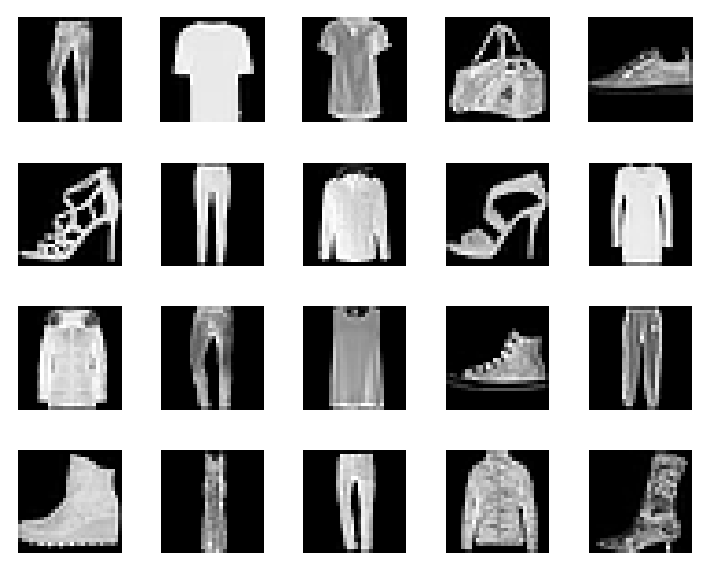
\includegraphics[width=.9\textwidth]{20-immagini-random.eps}}
    \caption{20 immagini casuali di capi di abbigliamento dal \emph{training set} di Fashion MNIST.}
    \label{fig:20immagini}
\end{figure}

\newpage
Abbiamo inoltre visualizzato un singolo elemento dal dataset, e abbiamo prodotto l'istogramma dei livelli di grigio di questa immagine (Figura~\vref{fig:istogramma}).

\begin{figure}[htp]
    \centering
\begin{subfigure}{.3\textwidth}
    \centering
    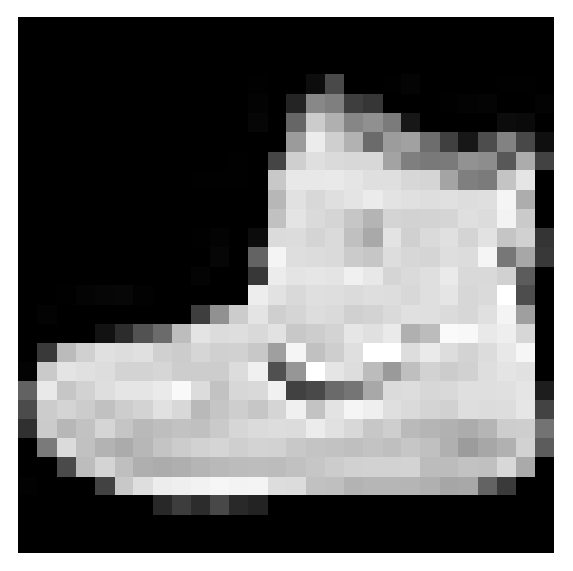
\includegraphics[width=.5\linewidth]{histogram-pic.eps}
\end{subfigure}%
\begin{subfigure}{.7\textwidth}
    \centering
    \tcbox[boxrule=.3mm,colback=white]{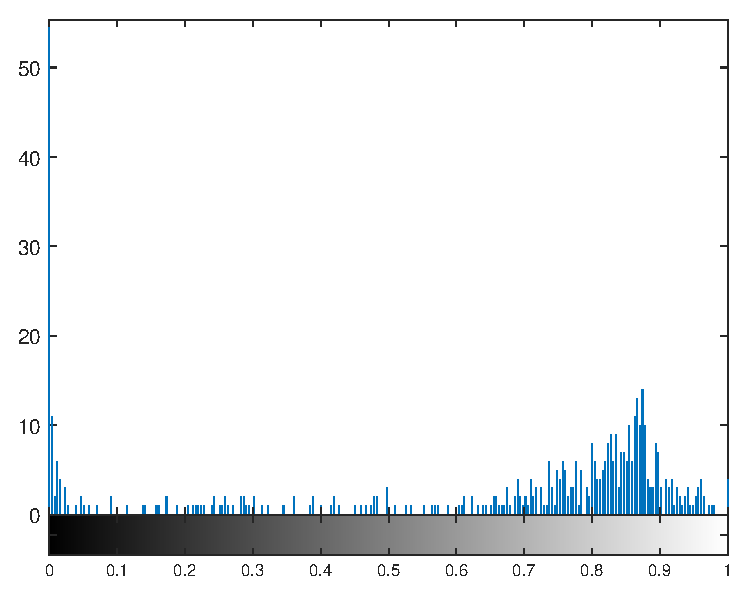
\includegraphics[width=.9\linewidth]{histogram.eps}}
\end{subfigure}

    \caption{Singola immagine del dataset FashionMNIST con l'istogramma dei livelli di grigio.}
    \label{fig:istogramma}
\end{figure}


\newpage 
\paragraph{5(c) Stima dell'errore MSE e visualizzazione delle curve.} Durante la procedura di apprendimento abbiamo calcolato e raccolto i dati necessari a tracciare delle curve \emph{loss}. In particolare, in Figura~\vref{fig:loss10} è riportata la \emph{loss curve} per 10 epoche, mentre in Figura~\vref{fig:loss100} la curva è relativa a 100 epoche. Entrambi gli addestramenti sono stati compiuti con un \emph{learning rate} pari a 0.01.

\begin{figure}[htb]
\center
    \tcbox[boxrule=.3mm,colback=white]{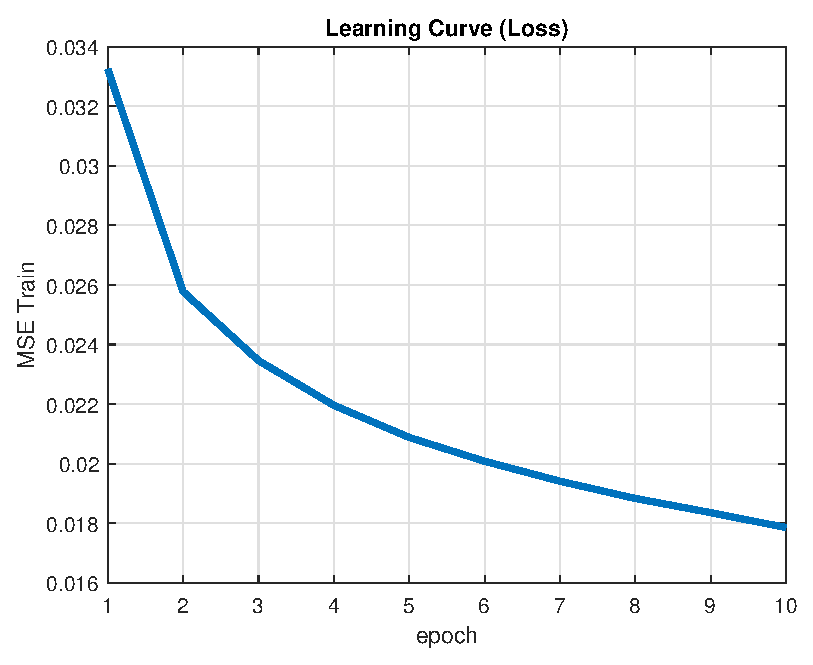
\includegraphics[width=.9\textwidth]{loss-10-epoch-0_01-alpha.eps}}
    \caption{Curva loss di apprendimento. \emph{Learning rate}: 0.01, epoche: 10.}
    \label{fig:loss10}
\end{figure}

\begin{figure}[htb]
\center
    \tcbox[boxrule=.3mm,colback=white]{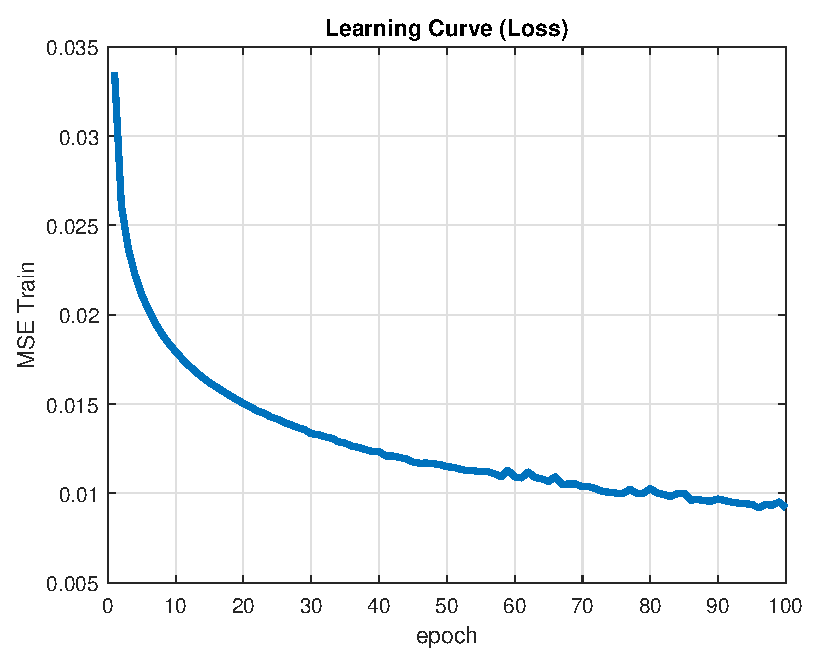
\includegraphics[width=.9\textwidth]{loss-100-epoch-0_01-alpha.eps}}
    \caption{Curva loss di apprendimento. \emph{Learning rate}: 0.01, epoche: 100.}
    \label{fig:loss100}
\end{figure}




\newpage ~ \newpage
%%%%%%%%%%%%%%%%%%%%%%%%%%%%%%
\section{Osservazioni e Conclusioni} % cap8

Nel \textbf{secondo} e \textbf{terzo capitolo} abbiamo presentato l'architettura della rete e come abbiamo strutturato il software. Nel \textbf{quarto} e \textbf{quinto} capitolo abbiamo descritto brevemente ma più in dettaglio le due procedure cardine di questo pacchetto: la funzione \texttt{FashionMNIST\_DataPrep} e lo script \texttt{FashionMNIST\_Training}. Nel \textbf{sesto capitolo} abbiamo riportato l'intero codice diviso per procedura, corredato di commenti.

Al \textbf{settimo capitolo} abbiamo presentato i risultati, che vengono qui discussi.

\paragraph{4(c) Esplorazione dei dati.}
in \texttt{FashionMNIST\_DataPrep} abbiamo visualizzato un sottoinsieme di venti immagini prese a caso nel \emph{training set} (Fig.~\vref{fig:20immagini}). Possiamo notare come queste immagini sono a bassa risoluzione; come già detto, la loro dimensione in pixel è $28\times28$. 

In particolare osserviamo i livelli di grigio, che sono pochi. A questo proposito abbiamo visualizzato una singola immagine con il relativo istogramma dei livelli di grigio (Fig.~\vref{fig:istogramma}). Abbiamo riscontrato come i 256 livelli non sono tutti popolati, e specificatamente si osservano dei picchi di densità di livelli in corrispondenza di una vicinanza al nero e al bianco. Questo, come risultato, non permette di valutare le sfumature dell'immagine, che sembra quasi una \emph{silhouette} dell'oggetto in questione.

Si può concludere che questo archivio di immagini è volutamente tenuto sia a bassa risoluzione che a basso intervallo di grigi per ridurre la complessità della rete naurale per la classificazione degli articoli.




\paragraph{5(c) Stima dell'errore MSE e visualizzazione delle curve.}
Abbiamo addestrato la rete utilizzando un \emph{training set} di 56 000 immagini scelte a caso dall'intero dataset FashionMNIST, e un valore di tasso di apprendimento pari a $0.01$. Durante l'apprendimento, ad ogni epoca abbiamo calcolato il \emph{mean squared error} tra l'\emph{output} della rete e il valore corretto. Con questi dati abbiamo tracciato la curva \emph{loss}.

Si può osservare come già dopo solo 10 epoche (Fig.~\vref{fig:loss10}) l'errore si abbassa al di sotto di un valore di $0.02$. Compiendo 100 epoche (Fig.~\vref{fig:loss100}) l'MSE scende ulteriormente, ma non di molto, fino a meno di $0.01$.

Concludiamo quindi che l'apprendimento è buono in quanto la curva di errore converge, ed è piuttosto rapido: sono necessarie una decina di epoche per ottenere un valore molto basso di errore.








\end{document}